\documentclass[12pt, twoside]{report}
\usepackage[spanish]{babel}
\usepackage[utf8]{inputenc}
\usepackage[T1]{fontenc}
\usepackage[final]{microtype}
\usepackage[letterpaper,width=170mm,top=25mm,bottom=25mm,bindingoffset=6mm]{geometry}
\usepackage{graphicx}
\graphicspath{ {images/} }
\usepackage{caption}
\usepackage{subcaption}
\usepackage{hyperref}
\usepackage[backend=biber,safeinputenc,sorting=none,backref=true]{biblatex}
\addbibresource{references.bib}
\usepackage{csquotes}
\usepackage{multirow}
\usepackage{afterpage}
\usepackage{pdflscape}
\usepackage[page, titletoc]{appendix}
\renewcommand{\appendixname}{Apéndice}
\renewcommand{\appendixtocname}{Apéndice}
\renewcommand{\appendixpagename}{Apéndice}

\usepackage{etoolbox} % utf8 encoding support for appendix
\makeatletter
\appto{\appendices}{\def\Hy@chapapp{Appendix}}
\makeatother

\usepackage{listings}
\captionsetup[lstlisting]{font={small,tt}}
\captionsetup[table]{name=Tabla}
\renewcommand{\floatpagefraction}{.8}
\newcommand\figlink[2]{\hyperref[#1]{en la Figura~\ref*{#1}{#2}}}
\newcommand\Figlink[2]{\hyperref[#1]{La Figura~\ref*{#1}{#2}}}
\newcommand\Fig[2]{\hyperref[#1]{(Fig.~\ref*{#1}{#2})}}

\lstset{
  basicstyle=\scriptsize,
  %frame=single,
  breaklines=true,
  breakatwhitespace=false
  extendedchars=true,
}

\begin{document}

% Front Matter
\begin{titlepage}
  \begin{center}
    
\includegraphics[width=0.1\textwidth]{ucv.png}\\
    Universidad Central de Venezuela\\
    Facultad de Ciencias\\
    Escuela de Computación\\

    \vfill

    \Large
    \textbf{Métodos y Técnicas para el Cálculo y la Visualización de Métricas de Historiales en Artículos de Wikis}

    \vspace{3cm}

    \normalsize
    Trabajo Especial de Grado\\ 
    presentado ante la Ilustre\\
    Universidad Central de Venezuela\\
    Por el Bachiller\\
    María Gabriela Caetano De Lima\\
    para optar al título de\\
    Licenciado en Computación

    \vspace{1cm}

    Tutor: Eugenio Scalise

    \vfill

    Caracas, Julio 2014

  \end{center}
\end{titlepage}


\chapter*{Resumen}
\input{chapters/abstract}

\tableofcontents

\listoffigures

\listoftables

% Main Matter
\chapter*{Introducción}
\input{chapters/introduction}

\chapter{Técnicas de Visualización de Historiales de Wikis}
Un wiki es una aplicación web que permite a los usuarios la adición, modificación o eliminación de contenido en colaboración con otros \cite{Wikipediad}. Dentro de las implementaciones de wiki existentes, el proyecto de enciclopedia Wikipedia es el más popular en Internet y una de las páginas web más grandes del mundo con más de 18 billones de visitas al mes y 30 millones de artículos en 287 idiomas \cite{Wikipediae}.  
A diferencia de las enciclopedias tradicionales, Wikipedia permite a cualquier usuario registrado o no la edición del contenido de sus artículos. Ningún usuario es considerado el dueño de un artículo, y su contenido no es vetado ni aprobado autoridad reconocida alguna. Es por ello que los editores deben ponerse de acuerdo sobre el contenido y estructura del artículo a través del consenso \cite{Wikipediae}. 

Para facilitar la colaboración, todos los artículos de Wikipedia tienen asociado un historial de revisiones, que permite a los editores restaurar contenido perdido y deshacer cambios no deseados. El historial de revisiones, es una página que contiene una lista de las ediciones realizadas sobre un artículo, que incluyen fecha y hora de cada edición, el nombre de usuario o IP del editor y un resumen de edición \cite{Wikipediac}.

Según Scalise, los sistemas basados en MediaWiki, como Wikipedia, no explotan propiedades presentes en los datos de los historiales; en particular, la evolución de cada artículo, la comunidad de usuarios participantes y la frecuencia de los cambios. Además enfatiza que carecen de una visualización gráfica de los datos \cite{Scalise2008a}. Esto último ha sido el objeto de estudio de muchas investigaciones.

La literatura sobre visualizaciones de historiales de Wikipedia contiene en general visualizaciones que pueden clasificarse en dos grupos. El primero de ellos se enfoca en el estudio de la interacción de los editores de un artículo mediante visualizaciones de redes \cite{Sabel2007a}\cite{Suh2007a}\cite{Keegan2012a}, mientras que el segundo se centra en el estudio de la evolución de las propiedades de los artículos mediante su visualización en series temporales \cite{Viegas2004a}\cite{Wattenberg2007a}\cite{Nunes2008a}. Estos trabajos han permitido analizar la dinámica y coordinación de los editores, como también la detección de patrones de actividad, conflicto y vandalismo. En general, han permitido alcanzar conclusiones importantes sobre el comportamiento de la comunidad colaborativa de Wikipedia. 

Otro grupo de trabajos realizó aplicaciones web cuya finalidad es monitorear el estatus del historial de un artículo.  Entre esos están el WikiDashboard \cite{Suh2008a} y una herramienta estadística integrada en Wikipedia \cite{Akawikipedia.orga}. A diferencia de las aplicaciones anteriores, que se enfocan en generar visualizaciones exploratorias de todo el historial, este grupo de aplicaciones se centró en crear un monitor de estatus de actividades recientes que mantuviera actualizados a los usuarios con el fin de mejorar la transparencia y responsabilidad social en artículos de Wikipedia. Ello se logra a través de visualizaciones que dan múltiples representaciones (líneas de tiempo, cromograma, listas de usuario, etc.) de la información reciente de manera resumida.

\section{History Flow}
Una de las primeras visualizaciones de historiales de Wikipedia fue History Flow \cite{Viegas2004a}, que plantea una herramienta de análisis exploratorio de datos efectiva para revelar patrones sobre el comportamiento de una comunidad colaborativa como Wikipedia. El objetivo de History Flow es garantizar la visualización inmediata de tendencias generales del historial de revisiones preservando los detalles para una exploración más minuciosa.

Para explicar el método, se plantea el siguiente escenario. Tres autores (María, Susana y Andrés) colaboran en la redacción de un artículo. A cada colaborador se le asigna un color que lo va a representar en la visualización. En primer lugar, María crea el documento y añade una cantidad de texto. Esta versión es reflejada como una “línea de versión” vertical, de color negro y con una longitud proporcional a la longitud del texto (Fig. \ref{fig1}a). En la siguiente versión, Susana agrega texto al final del documento sin modificar lo hecho por María. La línea de versión ahora mostrará una sección de color blanco (correspondiente a Susana) debajo de la sección de María. De esta forma, la línea de revisión aumenta su longitud en esta versión para reflejar el crecimiento del documento.

\begin{figure}[ht]
  \centering
  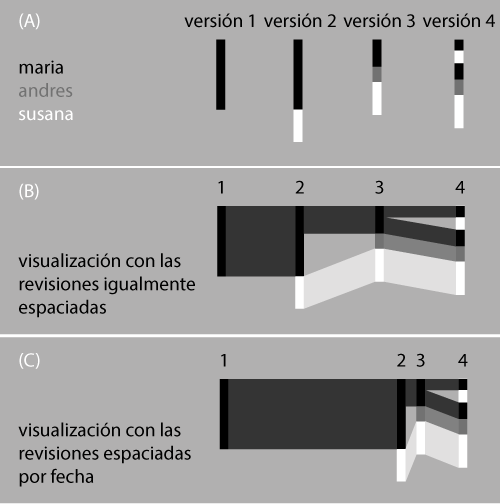
\includegraphics[width=0.75\textwidth]{fig1.png}
  \caption{Explicación del mecanismo de visualización History Flow}
  \label{fig1}
\end{figure}

En la versión 3, Andrés elimina una porción del texto original de María e introduce una pequeña contribución entre los textos de María y Susana. Finalmente, en la versión 4 Susana agrega texto en el medio de lo que resta del contenido de María.

Con el fin de observar las relaciones entre las diferentes versiones, el diagrama de History Flow vincula la sección de texto que se ha mantenido igual entre versiones consecutivas. Esto se logra dibujando conexiones sombreadas entre segmentos correspondientes a líneas de versión adyacentes, como se ve en la Fig. \ref{fig1}b. Los segmentos de texto que no tienen correspondencia en versiones adyacentes no se conectan y por ello el usuario observa el vacío en la visualización, destacando así claramente las inserciones y eliminaciones.

Una variante del History Flow emplea el espacio entre las líneas de revisión para reflejar el paso del tiempo. De esta forma, en lugar de utilizar el mismo espaciado entre líneas de revisión (Fig. \ref{fig1}b) se coloca un espaciado proporcional a la diferencia entre fechas de revisiones sucesivas (Fig. \ref{fig1}c). Esta variante tiene el beneficio de revelar los ritmos de colaboración entre autores.

\section{Chromogram}
El Cromograma es una técnica de visualización empleada por Wattenberg y Viegas \cite{Wattenberg2007a} para investigar la distribución del tiempo de los participantes de la comunidad colaborativa de Wikipedia. Consiste esencialmente en una visualización exploratoria que hace una codificación cromática de largas secuencias textuales, produciendo una visualización densa en datos que puede contener la vasta historia de ediciones de un usuario en una pantalla. Esta visualización permitió la identificación de patrones de actividades reactivas y sistemáticas en la comunidad colaborativa de Wikipedia.

El criterio de codificación toma las primeras tres letras para determinar el color de la representación. La primera letra determina el tono, la segunda la saturación y la tercera el brillo. Se restringe el rango de la saturación y el brillo de manera que el tono pueda percibirse fácilmente. Como caso especial, se codifican en escala de grises los títulos o comentarios que comienzan con un número.  La Fig. \ref{fig6} muestra ejemplos de esta codificación usando palabras comunes encontradas en los comentarios de los usuarios de Wikipedia.

\begin{figure}[ht]
  \centering
  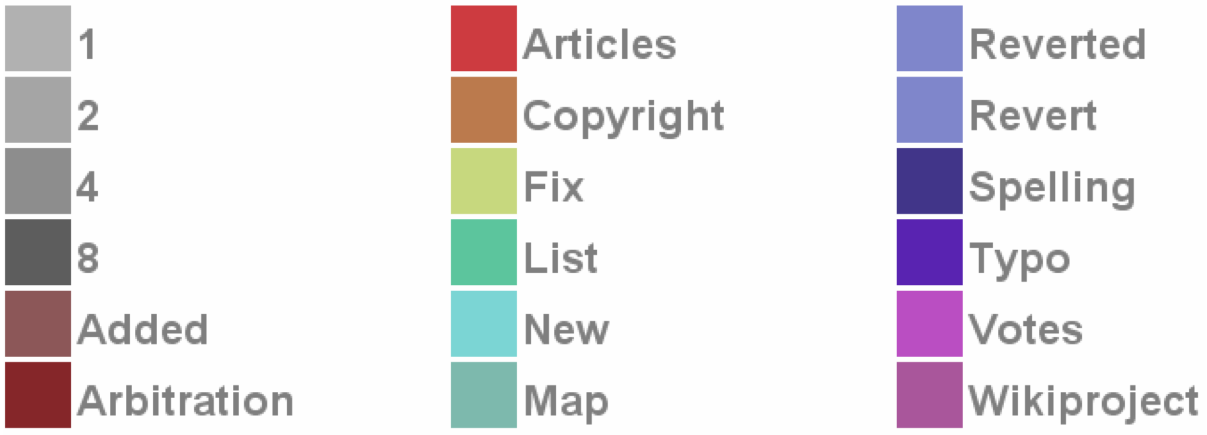
\includegraphics[width=0.75\textwidth]{fig6.png}
  \caption{Codificación de palabras a color}
  \label{fig6}
\end{figure}

La técnica del Cromograma parte de esta codificación y permite visualizar una larga historia de revisión en una sola pantalla. Para explicarla, en primer lugar se muestra en la Fig. \ref{fig7}a una lista hipotética de revisiones. La visualización consiste entonces en tomar el texto del comentario de cada elemento de la lista, codificarlo y crear un histograma (Fig. \ref{fig7}b) donde cada fila corresponde a un día y contiene un rectángulo para cada revisión ordenada en el tiempo. La Fig. \ref{fig7}c muestra la variante de la visualización llamada “vista de bloque”, donde las revisiones se muestran de manera continua y consolidada ordenadas en el tiempo de izquierda a derecha y luego de arriba a abajo. Esta vista es más densa, pero oculta los ritmos temporales de las revisiones.

\begin{figure}[ht]
  \centering
  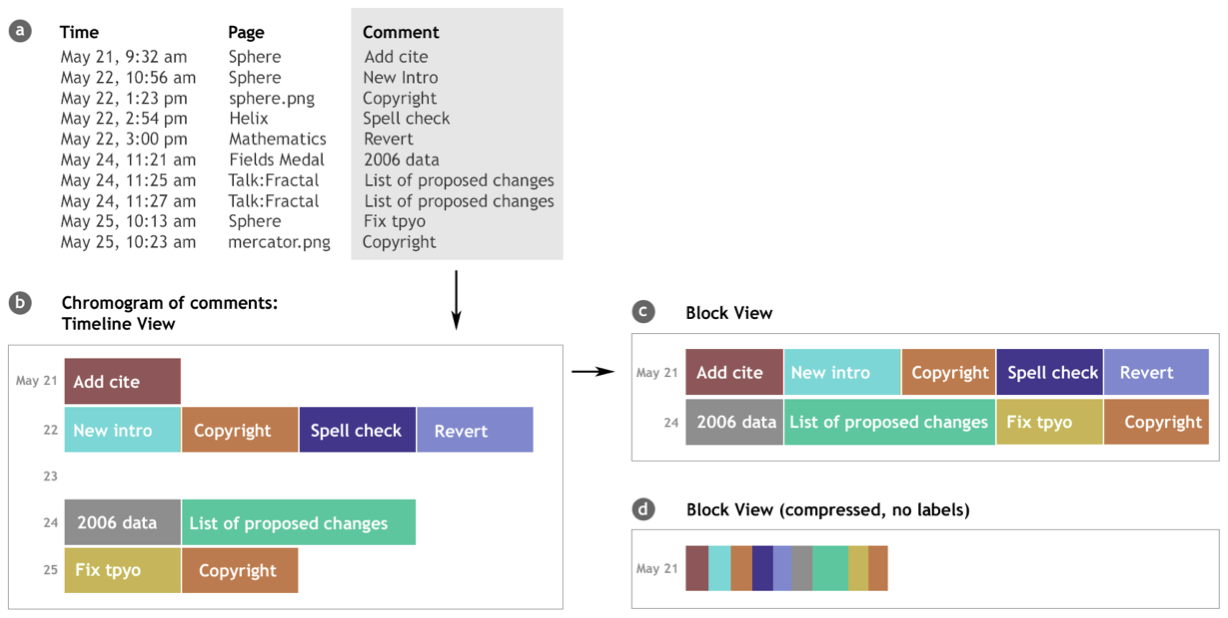
\includegraphics[width=0.75\textwidth]{fig7.png}
  \caption{Creando un Cromograma}
  \label{fig7}
\end{figure}

\section{WikiChanges}
Es una aplicación web diseñada con la finalidad de estudiar la correlación entre la popularidad de un tema y el perfil de actualización. Esto se logra mediante una visualización que gráfica sobre una línea de tiempo el número de revisiones que sufre un artículo, acompañado de un resumen de revisiones que crea una nube términos que ayuda a determinar los eventos asociados a picos de actividad.

Según el autor, el perfil de actualización es “la distribución de revisiones en el tiempo hecha sobre un artículo en un sistema de wiki”. Para construir el perfil de actualización de un artículo de Wikipedia, se extrae la fecha de cada revisión, se cuenta el número de revisiones por período (día, mes o año) y se produce una serie de tiempo.
En la Figura \ref{fig10}, se muestra el perfil de actualización del artículo sobre Steve Fossett. Se puede observar un pico de actividad en Septiembre del 2007, fecha en la cual fue reportado desaparecido durante un vuelo, y luego otro en Febrero del 2008 cuando fue declarado muerto. Dado que en este caso se conocen de antemano los eventos asociados al artículo, es fácil predecir y entender los picos de actividad. Sin embargo, cuando estos eventos asociados no se conocen, la visualización por sí sola no permite descubrir las posibles causas de los picos de actividad. Como solución a esta limitante, se planteó la construcción automática de “resúmenes”.

Estos resúmenes se construyen para un período dado usando un enfoque basado en los términos insertados entre revisiones. Sólo se considera la versión más antigua y la más reciente del documento analizado en el período definido. De cada versión se prepara un conjunto de términos acompañados de su frecuencia. Los términos pueden ser una palabra (unigrams) o  la ocurrencia de dos palabras consecutivas (bigrams). Sustrayendo la frecuencia de los términos en la versión más antigua de la más reciente obtenemos el conjunto que formará la nube de términos para el período determinado. Cada término es ponderado usando su frecuencia resultante, como se muestra en la Fig. \ref{fig10}.

\begin{figure}[ht]
  \centering
  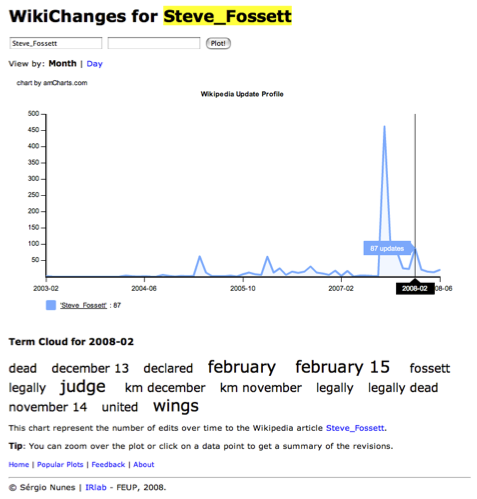
\includegraphics[width=0.75\textwidth]{fig10.png}
  \caption{Sistema WikiChanges mostrando la historia de revisiones para el artículo de Steve Fossett}
  \label{fig10}
\end{figure}

\section{Revert Graph}
En este trabajo se describió un modelo para identificar patrones de conflicto en artículos de Wikipedia. El modelo se basa en el historial de ediciones de usuarios y las relaciones entre sus ediciones, especialmente aquellas que eliminan ediciones previas; conocidas como “reversiones” o “reverts”. Basados en este modelo, se construyó Revert Graph, una herramienta que utiliza grafos de nodos para visualizar patrones de conflicto generales entre grupos de usuarios.
 
Se plantean dos métodos para identificar “reversiones” en Wikipedia. El primero se basa en calcular un identificador único para cada revisión en un artículo usando un esquema de hashing MD5. Se usa la función de MD5 para generar una pequeña huella digital de cada revisión, la cual permite una rápida comparación entre todos los artículos. El segundo método permite capturar las “reversiones” parciales usando las etiquetas “revert” y “rv” en los comentarios del editor en cada revisión.

Inicialmente, la herramienta carga un grupo de usuarios participando en la edición de un artículo como un grafo de nodos uniformemente distribuido. La simulación ejecuta un algoritmo de disposición que simula la dinámica social que resulta del modelo de conflicto de usuarios. Este algoritmo asigna fuerzas tal que los bordes (que representan relaciones de reversión) funcionan como resortes, mientras que los usuarios son representados como partículas con campos gravitacionales. A medida que la simulación progresa, las fuerzas del grafo se estabilizan y las estructuras sociales entre usuarios empiezan a emerger, como se muestra en la Figura \ref{fig11}. El tamaño del nodo es proporcional al número de reversiones o revisiones. Los nodos son codificados con color basándose en el estatus de registro de los usuarios. Un administrador se colorea como un nodo verde, un usuario registrado normal como uno gris y uno no registrado como uno blanco.

\begin{figure}[ht]
  \centering
  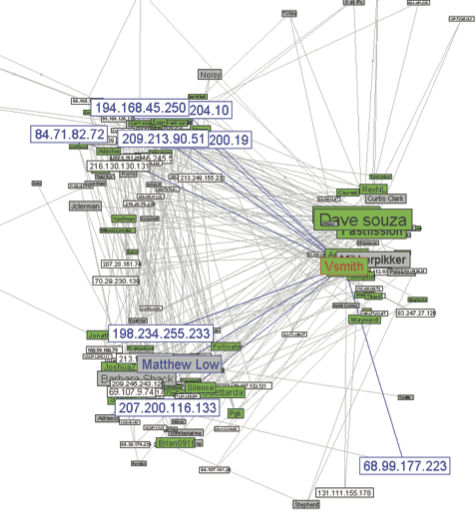
\includegraphics[width=0.75\textwidth]{fig11.png}
  \caption{Visualización Revert Graph del artículo de Charles Darwin}
  \label{fig11}
\end{figure}

\section{Estructuras y Dinámicas de las Colaboraciones en Wikipedia en Eventos Recientes}
Este trabajo estudia la dinámica de coordinación de los editores de Wikipedia sobre dos categorías de artículos: aquellos sobre eventos recientes y aquellos que son enciclopédicos. Los resultados mostraron que las estructuras y dinámicas son distintas entre artículos para estas dos categorías y que tienen implicaciones en cómo los sistemas de inteligencia colectiva pueden apalancarse para procesar y dar sentido a información compleja.

La visualización emplea una perspectiva de análisis de red. Este enfoque se basa en la construcción de una “trayectoria de artículo”, que es la secuencia temporal de las revisiones contenidas en el historial. Los nodos en la trayectoria son los autores, mientras que las conexiones entre nodos representan las revisiones que transicionan el artículo de la revisión de un autor a la del siguiente. Un lazo ocurre cuando un solo editor guarda múltiples revisiones a lo largo del historial de un artículo (Fig.\ref{fig12}). Una cadena aparece cuando editores subsecuentes hacen revisiones únicas sin contribuir nuevamente en el artículo (Fig. \ref{fig13}). En general, esta técnica captura una vista estructural de la historia de revisiones que permite visualizar y analizar relaciones complejas entre editores y las versiones de un artículo.

\begin{figure}
  \begin{subfigure}[b]{0.5\textwidth}
    \centering
    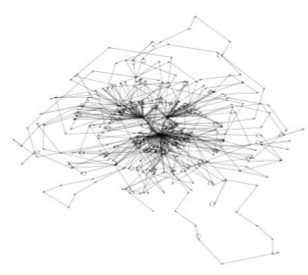
\includegraphics[width=0.75\textwidth]{fig12.png}
    \caption{Visualización de lazo}
    \label{fig12}
  \end{subfigure}
  \hfill
  \begin{subfigure}[b]{0.45\textwidth}
    \centering
    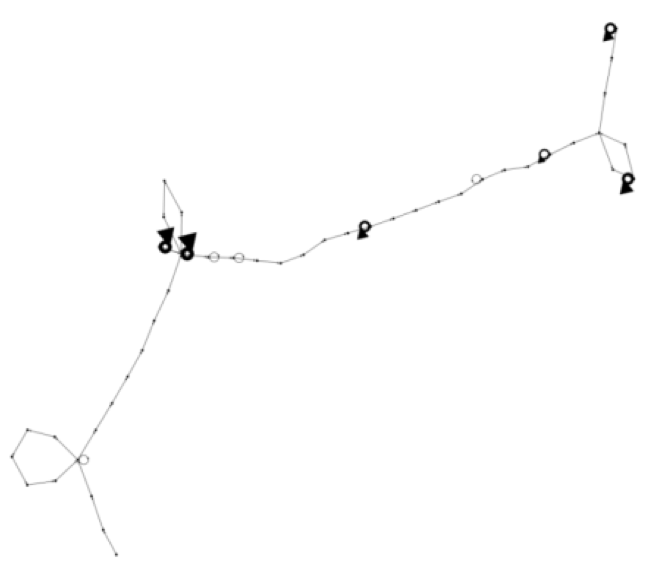
\includegraphics[width=0.75\textwidth]{fig13.png}
    \caption{Visualización de cadena}
    \label{fig13}
  \end{subfigure}
\end{figure}

\section{Visualización de Propiedades de Historiales de Artículos de Wikis Mediante un Enfoque de Ingeniería Dirigida por Modelos}
En el trabajo de Scalise se describe un enfoque dirigido por modelos para el procesamiento del historial de los artículos de un sistema Wiki basado en MediaWiki \cite{Scalise2008a}. En él se describe cómo se pueden calcular propiedades alternas a las disponibles, así como la generación de reportes y visualizaciones gráficas de la información. El proceso se compone de cuatro fases.

En la primera se define un metamodelo del dominio. En la segunda fase se genera un mecanismo para convertir los historiales en un modelo conforme con el metamodelo definido. En la tercera fase se hace uso del modelo para desarrollar transformaciones que  calculen propiedades sobre los datos. Se definen tres tipos de propiedades: generales, con clasificador y específicas. Las generales son propiedades numéricas (enteras o reales) calculadas para un artículo. Las propiedades con clasificador son aquellas similares a las generales, pero que agrupan o discriminan por una condición denominada clasificador. Las propiedades específicas son aquellas orientadas a visualizaciones particulares o reportes de los datos gestionados por el Wiki. Se cita como ejemplo de propiedad específica la calculada para la generación del gráfico History Flow.

En la cuarta fase se generan reportes o representaciones gráficas con las propiedades (métricas) calculadas. En el trabajo se hacen las siguientes recomendaciones en ese sentido:

\begin{itemize}
  \item Si se desean comparar las propiedades generales entre distintos artículos del Wiki, resulta apropiado los reportes mediante tablas o diagramas de barras.
  \item Si la visualización corresponde a propiedades con clasificador, entonces se recomiendan reportes textuales en forma de tablas y diagramas de torta (pie charts) para visualizar porcentajes.
\end{itemize}

Para la visualización de propiedades generales y con clasificador, se siguió un enfoque en el cual se escoge el metamodelo de visualización apropiado y luego se escribe la transformación para generar la instancia con los datos del historial del wiki. Por último se importan los resultados hacia cualquier herramienta de visualización utilizando una transformación.

En el ámbito de las propiedades específicas, se desarrolló una adaptación del gráfico History Flow, denominada History Graph. La estrategia usada para implementar esta visualización fue definir el metamodelo, como se muestra en la figura de abajo, y luego escribir una transformación a partir de los datos traídos de MediaWiki. En general, las propiedades específicas no siguen ningún patrón. A causa de ello, es necesario definir un metamodelo particular para cada propiedad.

El trabajo concluye que la propuesta planteada permite recuperar información del web siguiendo un enfoque flexible, que disminuye las dependencias de los programas con respecto a los aspectos de formato y separa el cálculo de las propiedades de su posterior visualización, lo cual trae el beneficio de permitir que una misma propiedad pueda ser visualizada de diferentes formas.

\section{Métodos y Técnicas para el Cálculo y Visualización de Métricas de Historiales de Artículos Wiki} En su trabajo, D’Apuzzo y Worwa implementan una aplicación (Web Scraper) que permite la recuperación del historial de los artículos de cualquier Wiki basado en MediaWiki, para luego calcular métricas y propiedades de interés asociadas a dicha información. El trabajo halla su motivación en la carencia de herramientas gráficas para el análisis y visualización de propiedades de los historiales que permitan observar su evolución en el tiempo.  Un Web Scraper es un programa automatizado que se encarga de visitar de manera sistematizada un conjunto de URLs con el fin de obtener información y/o realizar actividades de rutina o mantenimiento (12). En este caso, se implementó un Web Scraper para la extracción de historiales de sistemas basados en MediaWiki con las siguientes políticas de selección, revisita y cortesía:

\begin{description}
  \item[Selección:] las URL a visitar son provistas por el usuario final; una a la vez, o por lote mediante un archivo de texto en el cual se especifica una URL por línea. Las URL suministradas son sometidas a un proceso de normalización.
  \item[Revisita:] la política de revisita se basa en un sistema de prioridades. Una URL recién almacenada tiene una prioridad de 0.5. Luego de visitada y de haber extraído la información, la prioridad se actualiza con el valor 0. Esta probabilidad irá aumentando en el tiempo de acuerdo a la formula:
\begin{equation}
  1-\frac{T_{0}}{T_{i}}
\end{equation}
donde To es la marca de tiempo (timestamp) de la última fecha de actualización de la URL (por defecto 0) y Ti es la marca de tiempo del momento en que se está calculando la prioridad de revisita.
  \item[Cortesía:] Se espera un tiempo mínimo de 10 segundos entre peticiones al servidor.
\end{description}

Como se muestra en la Figura \ref{fig16}, la arquitectura del Web Scraper incluye dos módulos de soporte: una herramienta de URL y un demonio de prioridades. La herramienta de URL es una pequeña aplicación que recibe como parámetro una URL, la normaliza y la agrega al sistema. El demonio de prioridades se encarga de la actualización del valor de prioridad de las URL almacenadas en la base de datos usando la fórmula establecida en la política de revisita.

\begin{figure}[ht]
  \centering
  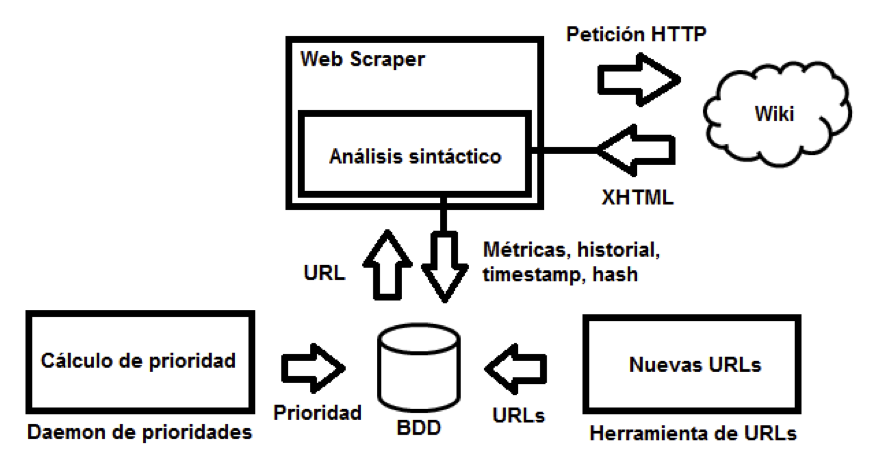
\includegraphics[width=0.75\textwidth]{fig16.png}
  \caption{Arquitectura del sistema WikiMetrics-UCV}
  \label{fig16}
\end{figure}

El funcionamiento del Web Scraper sucede de la siguiente manera. Dado el pool de semillas almacenadas en la base de datos por la herramienta de URLs, el Web Scraper selecciona la URL a visitar y se descarga el documento HTML. El documento pasa por un proceso de análisis sintáctico mediante el cual se extrae toda la información especificada por el usuario usando expresiones XPath. Está información es luego normalizada y almacenada en la base de datos.

La aplicación se implementó en lenguaje Python en combinación con una base de datos NoSQL manejada con MongoDB. Dicho proyecto se encuentra hospedado en la siguiente dirección de GitHub \url{https://github.com/bworwa/wiki_metrics_ucv}.



\chapter{Visualizaciones de Datos}
Según Kirk \cite{Kirk2012}, la visualización de datos es un proceso de diseño mediante el cual se codifican y presentan los datos de tal forma que se aprovechan las capacidades de percepción visuales para maximizar la efectividad y eficiencia con la que nuestro cerebro procesa información y produce conocimiento.

Según Ilinnsky y Steele \cite{Iliinsky2011a}, la visualización es un medio útil para examinar, entender y transmitir la información por diversas razones, entre las cuales están:

\begin{itemize}
  \item Aprovechar las capacidades de los sistemas visuales para transmitir una gran cantidad de información al cerebro rápidamente.
  \item Hacer uso de las capacidades del cerebro para identificar patrones y comunicar relaciones y significados.
  \item Inspirar mayores exploraciones y nuevas preguntas.
  \item Ayudar a identificar sub-problemas.
  \item Identificar tendencias y valores extremos, descubrir o buscar puntos de interés en un mar de datos, etc. 
\end{itemize}

Una función clave de la visualización de datos es mover información del punto A al punto B. En la visualización exploratoria de datos el punto A son los datos y el punto B es la mente del diseñador. En la visualización explicativa el punto A es la mente del diseñador y el punto B es la mente del usuario.

\section{Clasificación}
Las visualizaciones de datos pueden clasificarse de diversas maneras. Kirk \cite{Kirk2012} establece clasificaciones según la intención de la visualización; función y tono. Por su parte, Ilinnsky y Steele \cite{Iliinsky2011a} proponen una clasificación según la complejidad de la visualización.

\subsection{Según su función}

Involucra la experiencia funcional que se puede crear entre el diseño, los datos y el usuario. Se disponen de las siguientes tres alternativas:

\begin{itemize}
  \item Cuando la función es explicar.
  \item Cuando la función es explorar.
  \item Cuando la expresión es la expresión visual.
\end{itemize}

\subsubsection{Cuando la función es explicar}

En este caso se trata de comunicar información al usuario mediante una narrativa enfocada y específica. Las visualizaciones de este tipo se conocen como visualizaciones explicativas.

\subsubsection{Cuando la función es explorar}

Las visualizaciones de este tipo, denominadas visualizaciones de exploración, ofrecen al usuario un ambiente de exploración visual de datos que le permite sacar sus propios patrones, relaciones, tendencias y conocimientos.

Una funcionalidad que permite generar una experiencia verdadera de exploración es la interactividad. Con ella el usuario es capaz de sumergirse en un reto dinámico de solución de problemas. Algunas de estas de funcionalidades son el filtrado, ordenamiento, selección (brushing), ajuste de variables y modificación de vista.

\subsubsection{Cuando la función es la expresión visual}

En este caso se hace uso de los datos como materia prima para la expresión artística. Esto difiere de los casos anteriores cuya finalidad es esencialmente informar.

\subsection{Según su tono}

Esta clasificación se enfoca en la respuesta emocional y en el tipo de estímulo que se está intentando crear. Existen dos tonos diferenciados.

Pragmático y analítico: son aquellas visualizaciones que se enfocan en la necesidad de un diseño que entregue una representación de datos de forma rápida, eficiente y precisa. En este caso, el objetivo principal es informar.
Emotiva y abstracta: son aquellas enfocadas en la experiencia estética que ilustra la historia general de los datos. En muchos casos sacrifican el nivel de detalle con el fin de generar un impacto emocional o hacer énfasis en un hecho. Sin embargo, preservan la visión general.

\subsection{Según su complejidad}

Esta clasificación categoriza las visualizaciones según el número de variables que representan. Por ejemplo, un gráfico de precio de acción (stock) contiene cuatro propiedades: fecha, precio, compañía y capitalización de mercado. Cada una es una dimensión distinta de los datos, que puede ser codificada por separado, usando una propiedad visual diferente.

\section{Proceso de Diseño}

Kirk \cite{Kirk2012} propone un proceso de diseño para la visualización de datos que incluye las siguientes fases: concepción del proyecto, análisis de los datos y diseño. El método pretende ser independiente de la tecnología y hace énfasis en la conceptualización, razonamiento y la toma de decisiones. Evita cualquier sentido de instrucción dogmática y se enfoca en ofrecer un conjunto de pautas generales. Se pretende que el método sea adoptado con flexibilidad, basado en el propio juicio y discreción.

\subsection{FASE I: Concepción del proyecto}

Antes de acometer cualquier proceso de diseño, se debe estar claro sobre la motivación que da origen al proyecto. Esto involucra identificar la audiencia y sus necesidades. Es también fundamental revisar cuidadosamente la intención del proyecto y cómo se define la función y tono de la visualización.

\subsection{FASE II: Análisis}

Esta fase consta de dos actividades. En la primera se adquieren, preparan y estudian los datos. En la segunda se lleva a cabo un análisis visual con el fin de descubrir las historias claves contenidas en los datos.

\subsubsection{Preparando y estudiando los datos}

Los datos son la materia prima de una visualización. Sin importar lo que se intenta o espera mostrar a través de la visualización, los datos son los que cuentan la historia. Un conjunto de datos incompletos, con errores o simplemente aburridos contaminan la visualización con las mismas propiedades. La tarea primordial como diseñador en esta fase es evitar que esto suceda. Esto se logra mediante la adquisición y el estudio de los datos con el fin de entender su condición, características y el conocimiento potencial que contienen. Los mecanismos de preparación y estudio de los datos componen el proceso que se describe a continuación.

\begin{enumerate}
  \item El primer mecanismo es la adquisición de los datos, donde la selección del lugar y método para adquirirlos quedan en manos del diseñador. Algunos de los métodos de obtención más comunes son:
  \begin{itemize}
    \item Adquisición a través de terceros
    \item Descarga desde el sistema de una organización
    \item Recolección y registro manual
    \item Extracción desde una API web
    \item Extracción desde una página web mediante un Web Scraper
    \item Extracción desde un archivo PDF
  \end{itemize}
  \item Una vez adquiridos los datos, se lleva a cabo un examen exhaustivo para evaluar el potencial de los mismos a la hora de cubrir las necesidades de la visualización. Este examen involucra evaluar la completitud y calidad de los datos.  \item Luego se estudia la estructura fundamental de los datos en función de los tipos de variables y sus rangos. Las variables pueden ser de los siguientes tipos:
  \begin{itemize}
    \item Categórica nominal
    \item Categórica ordinal
    \item Cuantitativa (intervalos)
    \item Cuantitativa (proporciones)
  \end{itemize}
  \item En función de las evaluaciones realizadas en los mecanismos anteriores se hacen las transformaciones necesarias para depurar y organizar los datos. Esta etapa involucra tratamientos como la eliminación de duplicados, limpieza de valores erróneos, sellado de los vacíos causados por datos faltantes, manejo de caracteres poco comunes, entre otros.
  \item En este mecanismo nos alejamos de la depuración de los datos y nos enfocamos en su preparación y refinación para su uso en el análisis y la presentación. Algunas de las acciones consideradas son:
  \begin{itemize}
    \item Dividir los valores de cualquier variable, por ejemplo extraer el año de un valor fecha
    \item Formar nuevas variables en función de la combinación de otras
    \item Convertir texto libre en palabras claves o valores codificados,
    \item Derivar valores a partir de otros, por ejemplo obtener el género del título (Sr. o Sra.)
    \item Crear cálculos para usar en el análisis, como por ejemplo proporciones porcentuales
    \item Remover los datos redundantes para los cuales no hay un uso planificado
  \end{itemize}
  \item El siguiente paso consiste en determinar el nivel de resolución con el que se necesita presentar los datos. Este proceso puede requerir agregar o desagregar datos para lograr el nivel correcto de detalles. A continuación se presentan las opciones disponibles para manejar la resolución de los datos:
  \begin{description}
    \item[Resolución completa:] consiste en trazar todos los datos disponibles con una marca individual
    \item[Resolución filtrada:] comprende la exclusión de registros en función a un criterio definido
    \item[Resolución agregada:] implica la agrupación de los datos por categorías especificas
    \item[Resolución muestral:] consiste en aplicar una regla de selección matemática particular para extraer una fracción de los datos. Es útil en la fase de diseño para probar las ideas.
    \item[Resolución global:] involucra presentar los totales estadísticos globales
  \end{description}
  \item El último mecanismo es el de consolidación. Se utiliza cuando se requiere de capas de datos adicionales para combinar con el conjunto de datos ya existente, realizar cálculos adicionales o simplemente acompañar los datos iniciales con el fin de crear contexto o mejorar el alcance de la comunicación.
\end{enumerate}

\subsubsection{Usando el análisis visual para encontrar historias}
El análisis visual de un conjunto de datos, mediante razonamiento inductivo y deductivo, permite al diseñador explorar los datos en todas las posibles direcciones. Haciendo uso de técnicas de visualización el diseñador puede familiarizarse íntimamente con los datos y comenzar a entender lo que se podría describir y cómo llevarlo cabo.

Durante el proceso de análisis visual se debe estar preparado para observar un conjunto de características (cualidades físicas de los datos) que servirán de guía en la identificación de historias claves. Estas características se describen en la siguiente tabla.
\begin{longtable}[c]{|p{3cm}|p{2.5cm}|p{3cm}|p{6.5cm}|}
  \hline
  Grupo & Visualización sugerida & Característica & Acción \\ \hline
  \multirow{4}{3cm}{Comparaciones y proporciones} & \multirow{4}{2cm}{gráfico de barras}
  & Rango y distribución & describir el rango de valores y la forma de la distribución de cada variable y combinación de ellas \\ \cline{3-4}
  &   & Clasificación &  estudiar el orden de los datos en función de la magnitud general\\ \cline{3-4}
  &   & Mediciones & ver más allá de la magnitud y estudiar el significado de valores absolutos \\ \cline{3-4}
  &   & Contexto & usar promedios, desviación, objetivos y predicciones como contexto para la evaluación de valores \\ \cline{3-4}
  \multirow{4}{3cm}{Patrones y tendencias} & \multirow{4}{2cm}{gráfico de líneas}
  & Dirección & descubrir la dirección en que cambian los valores (creciente, decreciente, constante) \\ \cline{3-4}
  &   & Tasa de cambio & estudiar la inclinación de los patrones de cambio \\ \cline{3-4}
  &   & Fluctuación & estudiar el ritmo y consistencia de los patrones de cambio mediante la observación de fluctuaciones significativas \\ \cline{3-4}
  &   & Significativo & determinar si los patrones que se observan son señales significativas o simplemente representan ruido dentro de los datos \\ \cline{3-4}
  &   & Intersección & estudiar las intersecciones y superposiciones entre las variables para determinar si el punto de cruce indica un cambio significativo en la relación \\ \cline{3-4}
  \multirow{4}{3cm}{Relaciones y conexiones} & \multirow{4}{2cm}{gráfico de dispersión}
  & Excepciones & identificar valores significativos que se encuentren por fuera de la norma, tal como los valores extremos que cambian la dinámica del rango de una variable \\ \cline{3-4}
  &   & Correlaciones & estudiar la evidencia de correlación fuerte o débil entre combinaciones de variables \\ \cline{3-4}
  &   & Asociaciones & descubrir las conexiones importante entre diferentes combinaciones de variables o valores \\ \cline{3-4}
  &   & Agrupaciones y vacíos & localizar los vacíos entre valores y las agrupaciones \\ \cline{3-4}
  &   & Relación jerárquica & determinar la composición, distribución y relevancia de las categorías de los datos \\ \cline{3-4}
  \hline
  \caption{Clasificación de las cualidades físicas de los datos}
  \label{tab1}
\end{longtable}

\subsection{FASE III: Diseño}
En esta sección se exponen las opciones de diseño involucradas en el proceso de creación de visualizaciones efectivas. Dichas opciones se separaran en dos capas:

\begin{itemize}
  \item Capa de representación de los datos, que es la capa primordial e involucra el cómo se le da forma a los datos a través del uso de variables visuales con el fin de construir gráficos y diagramas. 
  \item Capa de presentación de datos, que consiste en el formato de entrega, la apariencia y síntesis de todo el diseño. Involucra la capa de uso de color, interactividad, anotaciones y disposición de todos los elementos.
\end{itemize}

\subsubsection{Capa de representación de los datos}

En esta capa el enfoque está en conseguir el equilibrio entre la elegancia de diseño que satisfaga la intención del trabajo y el comportamiento funcional requerido para transmitir la información efectivamente. Para llevar esto a cabo se debe considerar lo siguiente:

\begin{itemize}
  \item La selección de un método de visualización adecuado para la historia que se va a contar
  \item El ajuste del diseño en función de las propiedades físicas de los datos
  \item La determinación de un grado deseado de precisión
  \item La creación de una metáfora visual apropiada para representar el tema de forma estilizada
\end{itemize}

\paragraph{Selección del método de visualización adecuado}

Consiste en determinar qué familia de métodos de visualización es la más adecuada para representar la historia que se va a contar. Existen varias formas de clasificar los métodos para visualizar datos. En la tabla XX se presenta una clasificación sugerida en función del método de narración principal.

\paragraph{Consideración de las propiedades físicas de los datos}

Ahora, el enfoque recae en encontrar el tipo de gráfico que se ajusta mejor a las variables de datos que se van a representar. La cantidad y naturaleza de las variables tendrán una influencia significativa al momento de reducir el rango de posibles tipos de gráficos que pueden ser utilizados dentro de la familia seleccionada en la tarea anterior.

%TO-DO: En la tabla XX… se presenta una lista de gráficos usando la taxonomía expuesta en la sección anterior…. (Descripción del cuadro…)

\paragraph{Determinación del grado de precisión en la interpretación}

La forma específica que se asigna a los datos para codificarlos visualmente se conoce como variables visuales. Una variable visual podría ser el largo o alto de una barra, la posición de un punto en el eje, el color de una ciudad en el mapa o la conexión entre dos nodos en una red. Los gráficos que conocemos como métodos de representación comunes se basan en el despliegue de una o combinaciones de varias variables visuales al mismo tiempo. Usar múltiples variables permite al diseñador expresar eficientemente capas extra de significado detrás de las propiedades de una sola marca. 

%TO-DO: Revisar y agregar bibliografía
Estudios como (Cleveland \& McGill (Journal of the American Statistical Association, Vol. 79, No. 387. September, 1984, pp. 531-554)) y (Jock Mackinlay) han demostrado como la efectividad de distintas variables visuales pueden ser jerarquizadas en base a la precisión con la cual soportan comparación y percepción de patrones. En la siguiente imagen (Image recreated from "Ranking of Perceptual Tasks" (Automating the Design of Graphical Presentations of Relational Information, ACM Transactions on Graphics, Vol.5, No.2, April 1986) by Jock MacKinlay.) se expone dicha jerarquía.

Estos estudios se enfocaron en el hecho de que nuestro sistema visual no es capaz de mediciones absolutas y por tanto, sólo se plantea una guía para entender cual variable va a ser mejor para entregar mediciones relativas con la mayor precisión.

\paragraph{Creación de una metáfora de diseño apropiada}
Una metáfora visual es una capa adicional de significado que se enfoca en transmitir un extra de conexión entre los datos, el diseño y el tema.

\paragraph{Selección de la solución final}
A partir de las opciones que procesamos en las tareas anteriores se puede identificar la especificación de la representación correcta de los datos para la visualización.

La clave es enfocarse en entregar los elementos funcionales apropiados mediante el uso de la representación de datos más adecuada para la visualización y dejar que la estética emerja como consecuencia de un buen diseño.

\subsubsection{Capa de presentación de los datos}
La presentación de los datos involucra las decisiones de diseño asociadas a todas aquellas características adicionales que podrían ser incluidas en la visualización. Estas son:

\begin{itemize}
  \item El uso del color
  \item La potencialidad de funciones interactivas
  \item Las anotaciones explicativas
  \item La arquitectura y disposición
\end{itemize}

Las decisiones que se hacen sobre estas capas deben enfocarse en proporcionar mayor significado, intuitividad y profundidad en la comprensión de los lectores o usuarios.

Uno de los conceptos claves para guiarse en la selección de opciones de diseño relacionadas con la presentación es hacer invisible aquello que es visible. Esto significa hacer que los elementos de presentación se sientan casi invisibles, tal que la ilustración de los datos preserve su dominio visual. En ese sentido, debe tenerse en mente dos cosas:

\begin{itemize}
  \item La inferencia visual se traduce en inferencia de datos.
  \item Los elementos visuales deben facilitar la discriminación de los datos.
\end{itemize}

\paragraph{El uso del color}

El mejor consejo para guiarse en el uso del color es asegurarse de que se usa de forma no intrusiva y que no conduzca erróneamente a interpretaciones cuando no debe. A continuación se muestran consideraciones para los siguientes tres casos de uso del color.

\subparagraph{Para representar datos}

Uno de los errores más comunes en el uso del color es el empleo de su propiedad del tono (hue) para representar datos cuantitativos. Esto es inapropiado ya que el ser humano no percibe un color como inherentemente más grande o pequeño que otro. Si se desea emplear el color para la representación de datos cuantitativos, es más efectiva la variación del brillo para un tono de color dado. A esto también se le conoce como esquema de color secuencial. Esta propiedad sí proporciona un sentido de los valores que son más altos y bajos, aunque es necesaria la incorporación de una leyenda que ayude a precisar valores absolutos. Más que obtener valores precisos, el sombreado de los patrones de mayor y menor valor es realmente el propósito principal del uso del color para representar datos cuantitativos.

Hay otros tipos de esquemas de color usados para situaciones que requieren la presentación de dos variables cuantitativas o para destacar los dos extremos de una sola variable. Éstos se conocen como esquemas divergentes, y por lo general presentan los extremos del espectro con colores oscuros y contrastantes.

Es importante tomar en cuenta que alrededor del 10\% de la población tiene una deficiencia en la percepción del color rojo y verde. Una alternativa efectiva en este caso es cambiar el verde por el azul.

Una de las funciones clave de una variable visual es facilitar la discriminación de los datos. El uso del tono de color para distinguir variables categóricas es particularmente efectivo. Sin embargo, es importante tomar en cuenta que el ojo es sólo capaz de distinguir hasta 12 clasificaciones de colores diferentes. El uso de una gama mayor puede dificultar la diferenciación de las distintas categorías.

\subparagraph{Traer los datos a un primer plano}

También se puede emplear el color para ayudar en la creación de un efecto de profundidad visual y una sensación de jerarquía en nuestros diseños. Básicamente se trata de traer los elementos más importantes a un primer plano y trasladar las menos importantes hacia el fondo. Un ejemplo de aplicación de esta técnica es el uso de un esquema de color monocromático que permita que otros tonos de color resalten al incorporarlos en aquellos aspectos que se quieren destacar.

En general, se recomienda no usar colores fuertes y altamente saturados al cubrir grandes áreas. En su lugar, es preferible usar estos colores para resaltar y llevar la atención a la capa de datos.

\subparagraph{Para adecuarse a requerimientos de diseño}

El factor final relacionado al color involucra la necesidad de incorporar la identidad visual de una organización mediante el uso de una paleta de color predefinida.

\paragraph{Creando interactividad}

Los avances de la tecnología en la última década han creado increíbles oportunidades para el desarrollo de poderosas visualizaciones interactivas. Los mejores diseños de interactividad se funden en el diseño de tal forma que el mecanismo de interacción es inseparable de la visualización de los datos.

El desarrollo de una visualización interactiva requiere de capacidades técnicas. Además, se debe tomar en cuenta la compatibilidad de la plataforma, la velocidad de carga de los datos y la capacidad del servidor.

La interactividad no siempre significa una experiencia de usuario mejorada. Por ello no se debe comprometer la esencia de la comunicación visual con el abandono del diseño estático por el simple hecho de crear interactividad. Un escenario apropiado para incorporar interactividad es cuando la complejidad y variedad de los datos son incompatibles con un diseño estático.

A continuación se muestra un resumen de la variedad de funciones y características que pueden considerarse en la construcción de una visualización interactiva.

\begin{description}
  \item[Manipulación de variables y parámetros:] es la habilidad de seleccionar, filtrar, excluir, o modificar ciertas variables para permitir al usuario interactuar con diferentes partes de los datos.
  \item[Ajuste de la vista:] tiene que ver con las capacidades de acercamiento del usuario hacia la visualización.
  \item[Animación:] es la inclusión de movimiento en la visualización. Esta técnica tiene gran potencial en datos basados en series temporales.
\end{description}

\paragraph{Anotaciones}

Las anotaciones ayudan a explicar y facilitan la experiencia visual e interpretativa. Es la capa de asistencia al usuario y de comprensión del usuario. Un objetivo clave del diseño de visualización de datos es facilitar la accesibilidad al tópico mediante un diseño intuitivo. El grado de accesibilidad se mejora con la inclusión de explicaciones útiles en todas las características de la visualización. No se debe asumir que el usuario podrá navegar con facilidad la visualización sin ninguna asistencia. Para ello se puede incluir con los siguientes elementos:

\begin{description}
  \item[Títulos:] pueden ayudar a atraer la atención de la audiencia y a articular el foco del tópico de la visualización.
  \item[Introducciones:] son importantes para explicar el trasfondo y contexto del proyecto.
  \item[Guías de usuario:] aunque la accesibilidad intuitiva es una meta fundamental, en algunos proyectos complejos es necesario hacer este tipo de anotaciones para dar mayor explicación al usuario.
  \item[Etiquetas:] revelan características extra y detalles sobre los datos.
  \item[Subtítulos y narrativa:] de manera complementaria con el título, estas anotaciones pueden ayudar a acelerar el proceso interpretativo y de compresión del usuario.
  \item[Anotaciones visuales:] son anotaciones que van más allá de ayudas textuales. Ejemplos de ellas son las cuadrículas, etiquetas de ejes, líneas de referencia y sombreado de fondo.
  \item[Leyendas:] explican los esquemas de color usados o los tamaños de las formas en términos de su representación categórica o cuantitativa.
  \item[Unidades:] deben incluirse detalles de las unidades de valor empleadas para evitar ambigüedades y malas interpretaciones.
  \item[Fuentes de los datos:] son referencias detalladas sobre dónde se obtuvieron los datos o cualquier otro elemento externo (como imágenes).
  \item[Atribuciones:] es el reconocimiento a personas que han contribuido directamente, influenciado la construcción del diseño o han servido de inspiración.
\end{description}

\paragraph{Disposición}

Es la capa final en la que se considera el acomodo del diseño en términos del formato, posicionamiento, y la organización de todos los elementos visibles. La intención con la disposición y arquitectura es proporcionar la experiencia más intuitiva posible. La meta es reducir la cantidad de trabajo que el ojo debe realizar para navegar en el diseño y descifrar la secuencia y jerarquía de la visualización. Deben considerarse con cuidado las elecciones en cuanto al tamaño, posicionamiento, agrupación y ordenamiento de todo lo que se muestre. Al igual que el resto de la capas de diseño, deben justificarse las decisiones de todas la propiedades visuales presentadas.

\section{La Práctica Gráfica}

En su libro "The Visual Display of Quantitive Information", Tufte \cite{Tufle2007a} postula los conceptos de excelencia gráfica e integridad gráfica, que son importantes como guías de evaluación de la calidad de una visualización de datos.

\subsection{Excelencia Gráfica}

La excelencia en los gráficos estadísticos consiste de ideas complejas comunicadas con claridad, precisión y eficiencia. Las visualizaciones deben:

\begin{itemize}
  \item Mostrar los datos.
  \item Inducir al usuario a pensar en la substancia en lugar de la metodología, diseño gráfico, tecnología o cualquier otra cosa.
  \item Evitar distorsionar los datos de cualquier manera.
  \item Presentar una gran cantidad de número en un espacio pequeño.
  \item Hacer coherentes un gran conjunto de datos
  \item Motivar al usuario a comparar diferentes trozos de datos.
  \item Mostrar los datos a distintos niveles de detalle, desde una visual amplia hasta la estructura fina.
  \item Servir a un propósito claro: descripción, exploración, tabulación o decoración.
  \item Estar integrado con la descripción estadística y verbal del conjunto de datos.
  \item Los gráficos "revelan" información sobre los datos.
\end{itemize}

\subsection{Integridad gráfica}

La integridad gráfica es el resultado de seis principios:

\begin{itemize}
  \item La representación de los números, deben ser proporcionales a las cantidades numéricas.
  \item Etiquetado minucioso, claro y detallado debe ser usado para atacar cualquier distorsión gráfica o ambigüedad.
  \item Mostrar variaciones en la data, no variaciones en diseño.
  \item El número de dimensiones mostradas no debe exceder el número de dimensiones de los datos.
  \item Los gráficos no deben citar datos fuera de contexto.
\end{itemize}




\chapter{Tecnologías para las Visualizaciones Web}
Las visualizaciones interactivas web se implementan combinando un conjunto variado de tecnologías: HTML para el contenido de la página, CSS para la apariencia, JavaScript para la interacción, SVG para los gráficos vectoriales, entre otros. Estas tecnologías funcionan de manera integrada sobre la representación compartida de la página llamada Modelo de Objetos de Documento (DOM) \cite{Bostock2011a}.

Actualmente existen toolkits que aprovechan estas tecnologías para la generación de visualizaciones de datos. El toolkit apropiado para cada caso debe seleccionarse tomando en consideración los requerimientos del proyecto, como por ejemplo el tipo de visualización, la tecnologías a usar, tiempo de desarrollo disponible y hasta la compatibilidad con navegadores, entre otros. Murray (2013) clasifica los toolkits disponibles de la siguiente manera:

\begin{itemize}
  \item Librerías de gráficos prediseñados
  \item Librerías para gráficos específicos (grafos, geomapping, etc.)
  \item Librerías para el diseño de visualizaciones 2D
  \item LIbrerías para el diseño de visualizaciones 3D
\end{itemize}

En este capítulo se presentan las más recientes especificaciones de las tecnologías fundamentales para la visualización, que incluyen HTML, CSS, DOM, scripting (JavaScript) y gráficos (PNG, SVG, Canvas, WebCGM). Por último se presentan aquellos toolkits que permiten el dibujo gráficos vectoriales sin limitarse a plantillas prediseñadas (D3.js, Processing.js, Raphael.js, Paper.js).

\section{Fundamentos tecnológicos}

\subsection{HTML}

HTML es el lenguaje de marcado para definir la estructura de las páginas web [w3c]. Está compuesto por elementos que definen el tipo de contenido que va a ser desplegado por el navegador y son a su vez estructuras semánticas que describen la función de cada parte del documento sin ambigüedad  [webplatform]. El estándar HTML es mantenido por W3C (World Wide Web Consortium) [mozilla:Introduction to HTML].

En un documento HTML un elemento se denota mediante un par de etiquetas, una inicial y otra final, como se muestra en la Figura \ref{sniphtml}. Un elemento puede contener otros elementos o texto. La información adicional asociada a un elemento se agrega mediante atributos colocados en la etiqueta inicial. En la Figura \ref{sniphtml} se muestra como se puede usar el atributo 'id' para proporcionar información semántica sobre el elemento.

%TO-DO: Soporte de lenguajes html, css, javascript y svg
\lstinputlisting[label=sniphtml,caption={Snippet de código HTML}]{snippets/snippet.html}

HTML5 es la quinta revisión del estándar HTML. Esta especificación intenta resolver las fallas que las anteriores tenían en el área de las aplicaciones web, ofreciendo un lenguaje de marcado y un conjunto de scripting APIs enfocados en la semántica [w3c:HTML5]. En cuanto al lenguaje de marcado, se introduce una conjunto de elementos y atributos nuevos entre los cuales están [W3C:HTML5-diff]:

\begin{itemize}
  \item Los semánticos, que son aquellos enfocados en mejorar la estructura del documento, como por ejemplo section, nav y header;
  \item Los multimedia, enfocados en eliminar las dependencias de plugins propietarios. Entre ellos están vídeo, audio y canvas;
  \item Los de formulario, que agregan un conjunto de valores (tel, email, url, color, etc.) al atributo 'type' del elemento 'input'. Esto mejora la experiencia de usuario ya que su entrada es validada antes  de ser enviada al servidor, reduciendo así el tiempo de respuesta.
\end{itemize}

Entre los APIs ofrecidos están aquellos para el control de video y audio, validación de formularios y el canvas 2D, entre otros [W3C:HTML5-diff]. El Canvas API es una tecnología de scripting que permite la creación y alteración de imágenes rasterizadas (bitmaps). Debido a que no tiene DOM, puede ejecutarse con bastante rapidez. Es soportado de manera nativa en la mayoría de los navegadores modernos en incluso en dispositivos móviles [w3c:webdesign/graphics].

\subsection{CSS}

Según la W3C CSS es un 'mecanismo sencillo para agregar estilo (tipografía, color y espaciado) a documentos web' [w3C:CSS]. Las hojas de estilo CSS ofrecen control sobre el formato y la disposición de un documento basado en XML. CSS trabaja sobre un sistema de reglas las cuales seleccionan un elemento que requiere de formato y luego establece valores a las diferentes propiedades del elemento [webplatform].

Una de las grandes ventajas de CSS es que permite la separación de estructura (HTML) y presentación (CSS), y con ello se simplifica el mantenimiento de una página, se promueve la reutilización de hojas de estilo y la se facilita la adaptación de páginas a diferentes entornos [w3c:HTML and CSS].

La sintaxis de CSS posee dos bloques básicos de construcción: la propiedad, que es un identificador, y el valor, el cual describe como esta propiedad debe ser manejada por el motor del navegador. La funcionalidad principal de CSS es de establecer un valor específico a una propiedad. Un par propiedad-valor se denomina declaración. El par es separado por dos puntos. Las declaraciones son agrupadas en bloques delimitados por llaves, mejor llamados bloques de declaración. Cada bloque de declaración está precedido por un selector que es una condición que selecciona algunos elementos de la página. El par selector-bloque de declaración es lo que se conoce como regla [developer.mozilla:css].

\lstinputlisting[label=snipcss,caption={Snippet de código CSS}]{snippets/snippet.css}

Las hojas de estilo pueden declararse dentro de un elemento HTML, dentro de la sección 'head' de un documento HTML o en un archivo CSS externo. Para determinar qué estilo va a ser usado cuando hay más de un estilo declarado para un mismo elemento HTML, se sigue lo que se conoce como orden de escascadamiento. En él los estilos prevalecen según el siguiente orden de prioridad ascendente [w3schools:css-howto]:

\begin{itemize}
  \item Estilo predefinido del navegador
  \item Hoja de estilo externa
  \item Estilos en la sección 'head' del documento HTML
  \item Estilos dentro del elemento HTML
\end{itemize}

CCS3 es la última revisión del lenguaje CSS y tiene como objetivo extender la especificación CSS2.1. Ofrece un conjunto de novedades como lo son los bordes redondeados, las sombras, las transiciones y nuevas plantillas de disposición. Permite adaptar la presentación de la página web a los distintos tipos de dispositivos [developer.mozilla: CSS3].

\subsection{DOM}

%TO-DO:(## Revisar: http://www.w3.org/TR/REC-DOM-Level-1/introduction.html; http://www.w3schools.com/dom/dom_intro.asp)

El modelo de objetos de documento (DOM) es una interfaz independiente de la plataforma y el lenguaje que permite a los programas y scripts el acceso dinámico y la actualización del contenido, estructura y estilo de documentos [w3c]. El DOM se crea al momento de cargar una página y es construido como un objeto con estructura de árbol[w3school], como se muestra en la Figura X. El DOM provee una representación del documento como una estructura de nodos que posee propiedades, métodos y manejadores de eventos. El DOM esencialmente conecta la página web a los scripts o lenguajes de programación [developer.mozilla/.../DOM].

%TO-DO: [agregar imagen del inspector]

\subsection{JavaScript}

Un script es un código de programa que no necesita de preprocesamiento (compilación) para su ejecución. En el contexto de un navegador web, el scripting se refiere por lo general a códigos de programa escritos en JavaScript que son ejecutados por el navegador cuando una página es descargada, o en respuesta a un evento provocado por el usuario [w3c: scripting].

JavaScript es un lenguaje interpretado, liviano, basado en prototipos y multiparadigma que soporta la programación orientada a objetos, imperativa y funcional [developer.mozilla/.../JavaScript]. 

JavaScript hace las páginas web más dinámicas al permitir modificar, agregar y enviar contenido desde la página sin tener que cargarla nuevamente. Adicionalmente, permite crear puentes de comunicación entre el navegador y la plataforma en donde corre, haciendo posible la incorporación de información local del ambiente del usuario [w3c:scripting].

Haciendo uso del DOM, JavaScript puede crear HTML dinámico de la siguiente manera [w3school]:

\begin{itemize}
  \item Cambiando los elementos HTML
  \item Cambiando los atributos HTML 
  \item Cambiando los estilos CSS 
  \item Eliminando elementos y atributos HTML existentes
  \item Añadiendo nuevos elementos y atributos HTML
  \item Reaccionando a eventos HTML 
  \item Creando nuevos eventos HTML
\end{itemize}

El siguiente es un ejemplo de una página HTML que haciendo uso de JavaScript muestra la fecha y hora local luego de presionar un botón.

\lstinputlisting[label=snipjs,caption={Snippet de código JavaScript}]{snippets/snippetjs.html}

\subsection{SVG}

SVG es el lenguaje de marcado XML para describir gráficos de aplicación e imágenes de 2 dimensiones y un conjunto de interfaces de scripts gráficos [w3c:svg].Comprende aspectos como la geometría de las formas, el estilo del texto, las animaciones y presentaciones multimedia (video, audio, etc.). Es totalmente interactivo y posee un DOM que permite scripting. Soporta un amplio rango de transformaciones visuales como gradientes, opacidad, filtros, recortes y máscaras [w3c:webdesign/graphics]. 

Usando SVG se pueden crear gráficos de alta calidad, completamente escalables y reusables; desde gráficos simples hasta potenciar páginas webs, desde diagramas interactivos hasta visualizaciones de datos. SVG es soportado por todos los browser modernos y está disponible para una gran variedad de dispositivos móviles [w3c:webdesign/graphics].

El siguiente es un ejemplo del uso de SVG para dibujar un círculo con un gradiente que simula el efecto de profundidad
\lstinputlisting[label=snipsvg,caption={Snippet de código SVG}]{snippets/snippet.svg}

\subsection{D3.js}

D3 es una librería de JavaScript que permite la inspección y manipulación directa del modelo de objetos del documento (DOM) [http://d3js.org/]. Fue desarrollada por Mike Bostock bajo la licencia BSD y se encuentra disponible en Github [InteractiveViz]. Con D3, el diseñador de manera selectiva vincula los datos de entrada a elementos arbitrarios del documento y luego aplica transformaciones dinámicas al contenido generado [D3-InfoVis]. Las transformaciones en D3 facilitan la implementación de visualizaciones dinámicas mediante control explícito de los elemento del modelo de objetos de dominio(DOM) y la evaluación inmediata de operadores sobre dichos elementos[D3-InfoVis].

D3 no es un framework monolítico que busca proveer todas las funcionalidades posibles. De lo contrario, se enfoca en la manipulación eficiente de un documentos en base a datos. Esto evita las representaciones propietarias y permite extraordinaria flexibilidad, exponiendo las capacidades de los estándares web como CSS3, HTML5 y SVG. D3 es extremadamente rápido, soporta grandes conjuntos de datos y comportamiento dinámico para interacciones. El estilo funcional de D3 garantiza códigos reusable y una amplia colección de componentes y plugins [http://d3js.org/].

\subsection{Raphael.js}

Es una librería de JavaScript para trabajar de manera sencilla con gráficos vectoriales en la Web [1]. Permite hacer tareas como crear gráficos personalizados, cortar imágenes y rotar widgets. Básicamente provee un API para la manipulación de SVG y el soporte de SVG para Internet Explorer [2]. Cada objeto que se crea es también un objeto DOM que puede modificarse posteriormente o adjuntársele manejadores de eventos de JavaScript. Esto permite la creación de visualizaciones interactivas y animaciones. Raphael soporta Firefox 3.0+, Safari 3.0+, Chrome 5.0+, Opera 9.5+ e Internet Explorer 6.0+.

%TO-DO: [[Agregar raphael_pic.jpeg, fuente: http://raphaeljs.com/github/dots.html]]

%[1] http://raphaeljs.com/
%[2] http://dev.opera.com/articles/raphael-javascript-api-for-svg/

\subsection{Processing.js}

Processing.js es la implementación web del popular lenguaje de programación Processing. Permite hacer visualizaciones de datos, arte digital, animaciones interactivas, gráficos educativos, juegos de video, entre otros, usando estándares web y sin necesidad de plugins [1]. Para usarlo simplemente se escribe el código en lenguaje de Processing (o su versión en JavaScript), se incluye en la página web y Processing.js se encarga de la implementación.La librería es compatible con cualquier navegador conforme con HTML5, incluyendo las versiones recientes de Firefox, Safari, Chrome, Opera e Internet Explorer.

Processing es un lenguaje de programación que consiste de un entorno de desarrollo, una colección de funciones y métodos, una sintaxis casi idéntica a Java y una comunidad en línea [2]. Un programa de Processing se llama un sketch, e implementa una programación escrita en Java que se siente más como el scripting, y que es más accesible a una audiencia más amplia que solo programadores, tales como artistas y diseñadores gráficos. 

%TO-DO: [[agregar pic, fuente: http://mattryall.net/blog/2008/11/wiki-visualisations-with-javascript]]

%[1] http://processingjs.org/
%[2] Visualizing Data_Exploring and Explaining - Ben Fry (p20)

\subsection{Paper.js}

Es un framework de código abierto para gráficos vectoriales que se ejecuta encima de HTML5 Canvas. Provee una interfaz de programación consistente y limpia con funcionalidades poderosas para crear y trabajar con gráficos vectoriales y curvas de bezier. Permite construir trayectorias y manipular sus curvas y segmentos de una manera conveniente y con gran precisión. Apunta a navegadores modernos que tengan soporte de Canvas y de ECMAScript5.


\chapter{Marco Metodológico}
\section{Motivación y Problema}

Actualmente, el manejador de wikis MediaWiki ofrece la posibilidad de consultar el historial de un artículo mediante una herramienta textual que permite visualizar los metadatos asociados a los cambios que ha sufrido un artículo (versiones). Adicionalmente, el historial de MediaWiki permite realizar comparaciones entre versiones y, si es necesario, revertir cambios.

Según Scalise \cite{Scalise2008a}, los sistemas como MediaWiki no explotan propiedades presentes en los datos de los historiales; en particular, la evolución de cada artículo, la comunidad de usuarios participantes y la frecuencia de los cambios. Además enfatiza que carecen de una visualización gráfica de los datos. Por ello planteó como solución el uso de técnicas de ingeniería de modelos para incorporar reportes alternos y visualizaciones sobre estos historiales. Esta solución dividió el proceso en tres actividades: extracción, cálculo de propiedades y visualización.

Una implementación del proceso propuesto por Scalise, con énfasis en la actividad de extracción, fue elaborada por D'Apuzzo y Worwa \cite{D`Apuzzo2012a} en la cual se creó una aplicación que permite recuperar historiales de artículos hospedados en MediaWiki (Web Scraper) acompañado de un Front-End sencillo para la visualización. En su estado actual, este Front-End permite visualizar un conjunto limitado de propiedades generales y es poco flexible en cuanto a las distintas gráficas que se pueden obtener de un mismo historial.
En este trabajo se propone superar estas limitaciones extendiendo el conjunto de métricas disponibles (incluyendo métricas específicas) y ofreciendo una gama de visualizaciones completa que incluya gráficos 2D y 3D.

\section{Objetivos del Trabajo}

El objetivo de este trabajo especial de grado es desarrollar un Front-End que permita visualizar propiedades asociadas a los historiales de artículos en Wikipedia.

Los objetivos específicos son:

\begin{itemize}
  \item Analizar y estudiar la aplicación WikimetricsUCV en su versión actual.
  \item Explorar el estado del arte en técnicas de visualización de datos.
  \item Escoger las tecnologías apropiadas para implementar una gama de visualizaciones flexibles e interactivas.
  \item Definir nuevas propiedades que puedan ser obtenidas a partir de los datos del historial de los artículos, haciendo uso del enfoque dirigido por ingeniería de modelos planteado Scalise.
  \item Definir una gama de visualizaciones flexibles e interactivas que permitan la detección de patrones, el análisis de la información a distintos niveles y se apoyen en el uso de una codificación visual efectiva.
  \item Diseñar e implementar un nuevo Front-End para la aplicación WikimetricsUCV.
\end{itemize}

\section{Estrategia de Solución}

\section{Tecnologías a Utilizar}

\section{Planificación Inicial del Proyecto}


\chapter*{Conclusiones}
\input{chapters/conclusion}

% Appendix
\begin{appendices}
  \chapter{Taxonomía de los Métodos de Visualización de Datos}
  \begin{longtable}{ | P{5cm} | P{5cm} | P{5cm} |}

    \hline
    \multicolumn{1}{|>{\columncolor[gray]{.5}}c|}{\bfseries Nombre} &
    \multicolumn{1}{|>{\columncolor[gray]{.5}}c|}{\bfseries Variables de Datos} &
    \multicolumn{1}{|>{\columncolor[gray]{.5}}c|}{\bfseries Variables visuales} \\
    \hline
  \endfirsthead

  \multicolumn{3}{|>{\columncolor[gray]{.8}}c|}{\bfseries Comparación} \\
  \hline
  Gráfico de puntos          & 1 categórica, 1 cuantitativa                        & Posición, color-tono, símbolo \\
  \hline
  Gráfico de barras          & 1 categórica, 1 cuantitativa-proporción             & Longitud/altura, color-tono \\
  \hline
  Gráfico de Gantt           & 1 categórica-nominal, 2 cuantitativa                & Posición, longitud \\
  \hline
  Gráfico de barras pixelado & Múltiples categóricas, 1 cuantitativa               & Altura, color-tono, símbolo \\
  \hline
  Histograma                 & 1 cuantitativa-intervalo, 1 cuantitativa-proporción & Altura, ancho \\
  \hline
  Gráfica de pendiente       & 1 categórica, 2 cuantitativa                        & Posición, conexión, color-tono \\
  \hline
  Gráfico radial             & Múltiples categórica, 1 categórica-ordinal          & Posición, color-tono, color-saturación/brillo, textura \\
  \hline
  Gráfico de glifo           & Múltiples categórica, Múltiples cuantitativa        & Forma, tamaño, posición, color-tono \\
  \hline
  Diagrama de Sankey         & Múltiples categórica, múltiples cuantitativa        & Altura, posición, enlace, ancho, color-tono \\
  \hline
  Gráfico de tamaño de área  & 1 categórica, 1 cuatitativa-proporción              & Área, color-tono \\
  \hline
  Gráfico de Trellis         & Múltiple categórica, Múltiple cuantitativa          & Posición, cualquier variable visual \\
  \hline
  Nube de palabras           & 1 categórica, 1 cuantitativa-proporción             & Tamaño \\
  \hline
  \multicolumn{3}{|>{\columncolor[gray]{.8}}c|}{\bfseries Jerarquía, relación partes a todo} \\
  \hline
  Gráfica de torta           & 1 categórica, 1 cuantitativa-proporción                 & Ángulo, área, color-tono \\
  \hline
  Gráfico de barras apiladas & 2 categóricas, 1 cuantitativa-ratio                     & Longitud, color-tono, posición, color-saturación/brillo \\
  \hline
  Gráfico de Waffle          & 1 categórica, 1 cuantitativa-proporción                 & Posición, color-tono, símbolo \\
  \hline
  Mapa de árbol              & Múltiples categórica-nominal, 1 cuantitativa-proporción & Área, posición, color-tono, color-saturación/brillo \\
  \hline
  Diagrama de empaquetado de círculos & 2 categórica, 1 cuantitativa-proporción        & Área, color-tono, posición \\
  \hline
  Jerarquía de burbuja       & Múltiples categórica, 1 cuantitativa-proporción         & Área, posición, color-tono \\
  \hline
  Árbol de jerarquía         & 2 categórica, 1 cuantitativa-proporción                 & Ángulo/área, posición, color-tono \\
  \hline
  \multicolumn{3}{|>{\columncolor[gray]{.8}}c|}{\bfseries Cambios en el tiempo} \\
  \hline
  Gráfico de línea           & 1 cuantitativa-intervalo, 1 cuantitativa-proporción, 1 categórica  & Posición, pendiente, color-tono \\
  \hline
  Minigráficas               & 1 cuantitativa-intervalo, 1 cuantitativa-proporción                & Posición, pendiente \\
  \hline
  Gráfica de área            & 1 cuantitativa-intervalo, 1 categória, 1 cuantitativa-proporción   & Altura, pendiente, área, color-tono \\
  \hline
  Gráfica de horizonte       & 1 cuantitiva-intervalo, 1 categórica, 2 cuantitativa-proporción    & Altura, pendiente, área, color-tono, color-saturación/brillo \\
  \hline
  Gráfico de área apilada    & 1 cuantitativa-intervalor, 1 categórica, 1 cuantitativa-proporción & Altura, área, color-tono \\
  \hline
  Gráfica de corriente       & 1 cuantitativa-intervalo, 1 categórica, 1 cuantitativa-proporción  & Altura, área, color-tono \\
  \hline
  Gráfico de barras (Candlestick chart) & 1 cuantitativa-intervalor, 4 cuantitativa-proporción    & Posición, altura, color-tono \\
  \hline
  Gráfico de código de barras & 1 cuantitativa-intervalo, 3 categóricas                           & Posición, símbolo, color-tono \\
  \hline
  Mapa de flujo              & Múltiples cuantitativa-intervalo, 1 categórica, 1 cuantitativa-proporción & Posición, altura/ancho, color-tono \\
  \hline
  \multicolumn{3}{|>{\columncolor[gray]{.8}}c|}{\bfseries Conexiones y relaciones} \\
  \hline
  Gráfica de dispersión      & 2 cuantitativa                                                 & Posición, color-tono \\
  \hline
  Gráfico de burbuja         & 2 cuantitativas, 2 categóricas                                 & Posición, área, color-tono \\
  \hline
  Matriz de gráficas de dispersión & 2 cuantitativa, 2 categórica                             & Posición, color-tono \\
  \hline
  Mapa de calor              & Múltiples categórica, 1 cuantitativa-proporción                & Posición, color-saturación \\
  \hline
  Conjuntos paralelos        & Múltiples categórica, múltiples cuantitativa-proporción        & Posición, ancho, enlace, color-tono \\
  \hline
  Red radial                 & Múltiples categórica, 2 cuantitativa-proporción                & Posición, conexión, ancho, color-tono, color-brillo, símbolo, tamaño \\
  \hline
  Diagrama de red            & Múltiples categórica, 1 cuantitativa-proporción                & Posición, conexión, área, color-tono \\
  \hline
  \multicolumn{3}{|>{\columncolor[gray]{.8}}c|}{\bfseries Mapeo geoespacial} \\
  \hline
  Mapa Chloropleth           & 2 cuantitativo-intervalo, 1 cuantitativo-proporción            & Posición, color-saturación/brillo \\
  \hline
  Mapa de puntos             & 2 cuantitativo-intervalo                                       & Posición \\
  \hline
  Mapa de burbujas           & 2 cuantitativo-intervalo, 1 cuantitativo-proporción, 1 categórica-nominal & Posición, área, color-tono \\
  \hline
  Mapa de contorno           & Múltiples cuantitativa, múltiples categórica                   & Posición, color-tono, color-saturación, color-oscuridad \\
  \hline
  Mapa de flujo de partículas & Múltiples cuantitativa                                        & Posición, dirección, grueso, velocidad \\
  \hline
  Cartograma                 & 2 cuantitativo-intervalo, 1 cuantitativa-proporción            & Posición, tamaño \\
  \hline
  Cartograma de Dorling      & 2 categóricas, 1 cuantitativa-proporción                       & Posición, tamaño, color-tono \\
  \hline
  Mapa de conexiones de red  & 2 cuantitativa-intervalo, 1 categórica-nominal                 & Posición, enlace, color-tono \\
  \hline
  \caption[Taxonomía de los métodos de visualización de datos]{Taxonomía de los métodos de visualización de datos}
  \label{table:appa}
 \end{longtable}

\end{appendices}

% Back Matter
\printbibliography

\end{document}
